
\chapter{Разработка программы решения теоретико-графовой задачи}
\label{cha:cppalgo}

\section{Задание}
\label{sec:cppalgo_task}

При выполнении этого этапа расчетной работы студенту необходимо
разработать и реализовать программу на С/С++, которая решает выданную
преподавателем теоретико-графовую задачу и соответствует следующим
требованиям:

\begin{itemize}
\item если преподаватель указал определенную структуру данных для
  представления графа, то в программе должна быть использована именно
  эта структура данных;
\item при своем запуске программа должна в автоматическом режиме
  стартовать 5 разнообразных примеров решения задачи и выводить
  результаты работы на консоль;
\item в программе должна оптимальным образом использоваться возможность
  языка программирования С/С++ по созданию функций;
\item в программе нельзя использовать глобальные переменные.
\end{itemize}

\section{Литература}

Начиная знакомство с полученной теоретико-графовой задачей, необходимо
поискать понятия, входящие в формулировку задачи, в
\href{http://pco.iis.nsk.su/grapp2/html/main.htm}{толковом словаре по
  теории графов}. В определении понятия в этом словаре есть ссылки на
соответствующую литературу. Также можно использовать словари по теории
графов на
\href{http://ru.wikipedia.org/wiki/%D0%A1%D0%BB%D0%BE%D0%B2%D0%B0%D1%80%D1%8C_%D1%82%D0%B5%D1%80%D0%BC%D0%B8%D0%BD%D0%BE%D0%B2_%D1%82%D0%B5%D0%BE%D1%80%D0%B8%D0%B8_%D0%B3%D1%80%D0%B0%D1%84%D0%BE%D0%B2}{Wikipedia}
и \href{http://mportal.narod.ru/Graphs/Search.html}{mportal.narod.ru}.

Основной литературой для выполнения расчетной работы является
следующий перечень книг:

\begin{itemize}
\item Оре О. Теория графов. — 2-е изд.. — М.: Наука, 1980. — С. 336.
\item Кормен Т. Х. и др. Часть VI. Алгоритмы для работы с графами //
  Алгоритмы: построение и анализ = Introduction to Algorithms. — 2-е
  изд.. — М.: Вильямс, 2006. — С. 1296.
\item Харари, Ф. Теория графов / Ф. Харари / Пер. с англ. и
  предисл. В.П. Козырева. Под ред. Г.П. Гаврилова. Изд. 2-е. – М.:
  Едиториал УРСС, 2003. – 269 с.
\item Нечипуренко, М. И. Алгоритмы и программы решения задач на графах
  и сетях / М.И. Нечипуренко, В.К. Попков, С.М. Майнагашев и др. –
  Новосибирск: Наука. Сиб. отд-ние, 1990. – 515 с.
v\item Емеличев В. А., Мельников О. И., Сарванов В. И., Тышкевич
  Р. И. Лекции по теории графов. М.: Наука, 1990. 384с. (Изд.2,
  испр. М.: УРСС, 2009. 392 с.)
\item Касьянов, В. Н. Графы в программировании: обработка,
  визуализация и применение / В. Н. Касьянов, В. А. Евстигнеева. –
  СПб. : БХВ-Петербург, 2003.
\end{itemize}

\section{Выбор среды разработки}

Рекомендую студентам в качестве среды разработки выбрать MS Visual
Studio. На мой взгляд, самым оптимальным выбором здесь будет MS Visual
Studio 2008 (или 9.0, что есть одно и то же). Образ диска-установщика
находится в папке
\verb|\\606srv\Install\~Development\~IDE\~MS Visual Studio\| и
называется <<\verb|MSVS_MSDN2008.iso|>>. На кафедре в учебных
лабораториях установлены MS Visual Studio 2003, 2008 и 2010.

Давайте рассмотрим процесс создания проекта в MS Visual
Studio. Запустите эту среду разработки и выберите пункт меню File ->
New -> Project. В диалоге <<New Project>> вас будет интересовать тип
проекта <<Win32 Console Application>> (как показано на рисунке
ниже). Выберите этот тип проекта и выведите название создаваемого
проекта и директорию, в которой он будет создан. Нажимайте <<OK>> и
будет открыт мастер создания данного типа проекта. В нем можно просто
нажать на кнопку <<Finish>>. Теперь с функции \lstinline{_tmain} (это
аналог знакомой вам функции \lstinline{main}) можно начинать писать
программу.

\textbf{Обратите внимание!} Заголовочный файл \verb|stdafx.h| является
\href{http://ru.wikipedia.org/wiki/%D0%9F%D1%80%D0%B5%D0%B4%D0%B2%D0%B0%D1%80%D0%B8%D1%82%D0%B5%D0%BB%D1%8C%D0%BD%D0%BE_%D0%BE%D1%82%D0%BA%D0%BE%D0%BC%D0%BF%D0%B8%D0%BB%D0%B8%D1%80%D0%BE%D0%B2%D0%B0%D0%BD%D0%BD%D1%8B%D0%B5_%D0%B7%D0%B0%D0%B3%D0%BE%D0%BB%D0%BE%D0%B2%D0%BA%D0%B8}{предкомпилированным}, поэтому во всех cpp-файлах инструкция \lstinline{#include "stdafx.h"} должна быть в самом начале файла (раньше нее можно помещать только комментарии).
 
  \begin{figure}[h!]
    \centering
    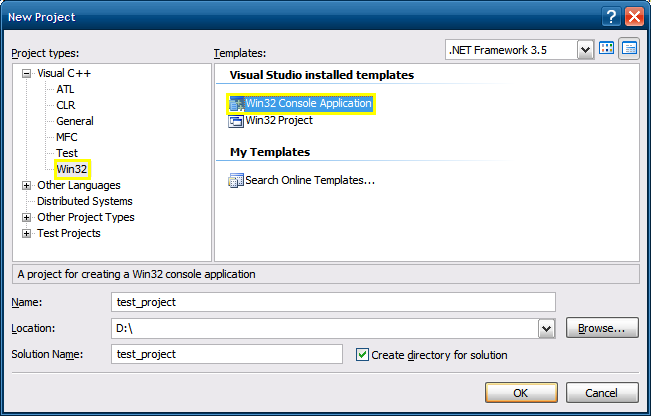
\includegraphics[scale=0.6]{1/Select_project_type}
  \end{figure}

Чтобы собрать проект, выберите пункт меню Build -> Build Solution
(Ctrl + Shift + B), затем выберите Debug -> Start Without Debugging
(Ctrl + F5) для запуска. Если хотите запустить под отладкой, то
выбирайте Debug -> Start Debugging (F5).

\section{Программа волнового поиска минимального пути}

\subsection{Описание алгоритма}

Алгоритм поиска одного из минимальных путей в неориентированном графе
является волновым и основан на понятии волны. В рамках этого алгоритма
волной называется множество вершин, каждая из которых является в
обрабатываемом графе смежной хотя бы одной вершине из предыдущей
волны. Волна, для которой нет предыдущей волны, называется начальной и
состоит из вершины, от которой начинается поиск минимального
пути. Волна, включающая конечную вершину пути, называется
конечной. Таким образом, наш алгоритм можно задать следующим перечнем
шагов:

\begin{enumerate}
\item Добавить все вершины графа, кроме начальной вершины пути, во
  множество непроверенных вершин.

\item Создать новую волну и добавить в нее начальную вершину пути.

\item Начальная волна – это новая волна. Новой волной будем называть
  последнюю созданную волну.

\item Сформировать следующую волну для новой волны. В нее попадет та
  вершина, которая является смежной вершине из новой волны и
  присутствует во множестве непроверенных вершин. Если вершина попала
  в формируемую волну, то ее надо исключить из множества непроверенных
  вершин. Созданную волну установить как следующую для новой волны, и
  после этого созданную волну считать новой волной.

\item Если новая волна пуста, то между вершинами не существует
  пути. Завершить алгоритм.

\item Если в текущей волне есть конечная вершина, то перейти к пункту
  7, иначе к пункту 4.

\item Сформировать один из минимальных путей, проходя в обратном
  порядке по списку волн. Завершить алгоритм.
\end{enumerate}

\subsection{Тестовые примеры}
\label{sec:cppalgo_tests}

1.  graph1.txt

\begin{figure}[h!]
  \centering
  
\includegraphics{1/test/1}
\end{figure}

2.  graph2.txt

\begin{figure}[h!]
  \centering
  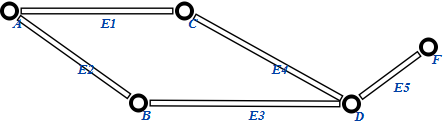
\includegraphics{1/test/2}
\end{figure}

3.  graph3.txt

\begin{figure}[h!]
  \centering
  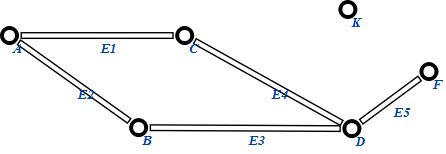
\includegraphics{1/test/3}
\end{figure}
 
4.  graph4.txt

\begin{figure}[h!]
  \centering
  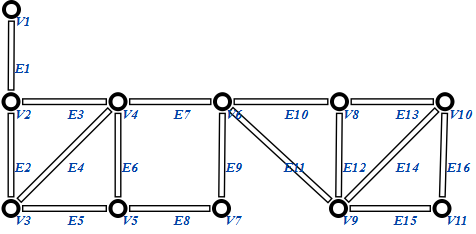
\includegraphics{1/test/4}
\end{figure}
 
5.  graph5.txt

\begin{figure}[h!]
  \centering
  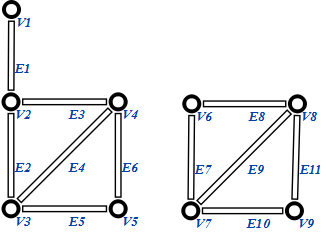
\includegraphics{1/test/5}
\end{figure}

\subsection{Создания программы}
\label{sec:Desc_prg}

%%% Local Variables: 
%%% mode: latex
%%% TeX-master: "ai_rr"
%%% End: 
